\section{Lockhart--McOwen Fredholm Theory on Manifolds with Ends}
\label{app:Fredholm}

\begin{remark}[Notation Reminder]
This appendix uses notation-heavy functional analysis. Recall from Remark~\ref{rem:NotationDisambiguation}: the exponent $\alpha$ (unsubscripted) denotes the Holder exponent in $C^{1,\alpha}$ regularity; $\alpha_{ind}$ denotes the positive indicial root of the stability operator; and $\beta, \delta, \tau$ are weight parameters in Sobolev spaces. The metrics are distinguished by their decorations: $g$ (initial data), $\bar{g}$ (Jang), $\tilde{g}$ (conformal), $\hat{g}_\epsilon$ (mollified).
\end{remark}

This appendix records the analytic background used in \S\ref{sec:Fredholm}.  The goal is to place the Lichnerowicz operator on the Jang manifold into the classical Lockhart--McOwen framework for elliptic operators on manifolds with ends.  The two inputs are: (i) the definition of the weighted Sobolev spaces adapted to the asymptotically flat and cylindrical regions, and (ii) the verification that the lower-order perturbations decay fast enough to be compact.

\subsection{Weighted Sobolev Spaces on the Ends}

Let $\mathcal{C} \cong [0,\infty)_t \times \Sigma$ denote a cylindrical end of $(\bM,\bg)$ and let $\rho$ be a defining function for the asymptotically flat end.  We employ the Lockhart--McOwen weighted Sobolev spaces
\[
    W^{k,p}_{\delta,\beta}(\bM) = W^{k,p}_{\delta}(\mathcal{E}_{AF}) \oplus W^{k,p}_{\beta}(\mathcal{C}) \oplus W^{k,p}(M_{\mathrm{bulk}}),
\]
where the AF norm uses the polynomial weight $\rho^{\delta}$ while the cylindrical norm uses $e^{\beta t}$ (or equivalently $\langle t \rangle^{\beta}$).  Explicitly,
\begin{equation}
    \|u\|_{W^{k,p}_{\beta}(\mathcal{C})}^p := \sum_{j=0}^k \int_{\mathcal{C}} e^{p\beta t} |\nabla^j u|^p_{\bg} \, dV_{\bg}.
\end{equation}
For $p=2$ these norms coincide with the Hilbert norms used in \S\ref{sec:Fredholm}, and the density/trace properties recalled there follow from the general theory in \cite{lockhartmccowen1985,melrose1996}.

\subsection{Compactness of the Potential Term}

\begin{lemma}[Decay of the Potential]\label{lem:PotentialDecay}
In the marginally stable case ($\lambda_1=0$) the potential term $V$ in $L = \Delta_{\bg} - V$ decomposes as $V = V_\infty + E(t)$ on each cylindrical end, where $|E(t,y)| \le C\langle t \rangle^{-4}$.  Consequently, multiplication by $E$ defines a compact operator
\[
    M_E : W^{2,p}_{\beta}(\mathcal{C}) \longrightarrow L^{p}_{\beta}(\mathcal{C})
\]
for every $p \in (1,\infty)$ and every $\beta \in \mathbb{R}$.
\end{lemma}

\begin{proof}
The decay estimate follows directly from the refined asymptotics of the Jang solution in the marginally stable case (see Han--Khuri \cite{hankhuri2013}, Theorem 1.2). Specifically, in the cylindrical coordinates $(t,y)$ where $t = -\ln s$, the metric components satisfy:
\[
    \bg_{tt} = 1 + O(t^{-2}), \quad \bg_{ty^a} = O(t^{-3}), \quad \bg_{ab} = \sigma_{ab}(y) + O(t^{-2}),
\]
with derivatives decaying one order faster, $\partial_t \bg \sim O(t^{-3})$.
The scalar curvature $R_{\bg}$ involves second derivatives of the metric. A direct computation in this chart shows:
\[
    R_{\bg} = R_{\sigma} - 2\partial_t^2 (\ln \sqrt{\det \bg}) - (\partial_t \ln \sqrt{\det \bg})^2 - \frac{1}{4}(\partial_t \bg_{ab})(\partial_t \bg^{ab}) + O(t^{-4}).
\]
Since the background cylinder has $R_{\sigma} = 0$ (or constant) and the perturbations are $O(t^{-2})$, the second derivatives are $O(t^{-4})$. Thus, the potential $V = \frac{1}{8}R_{\bg}$ satisfies
\[
    |V(t,y) - V_\infty| \le C t^{-4}.
\]
To prove compactness of the multiplication operator $M_E$, let $\{u_j\}$ be a bounded sequence in $W^{2,p}_\beta(\mathcal{C})$. By the Rellich--Kondrachov theorem, $u_j$ converges strongly in $L^p_{loc}$ on any finite cylinder $[0,T]\times \Sigma$. On the tail $[T,\infty)$, the decay of the potential gives uniform control:
\[
    \|E u_j\|_{L^p_\beta([T,\infty))} \le \sup_{t\ge T} |E(t)| \cdot \|u_j\|_{L^p_\beta} \le C T^{-4} \|u_j\|_{W^{2,p}_\beta}.
\]
Since $T^{-4}$ can be made arbitrarily small, the tails are uniformly negligible. Combined with local compactness, this proves $M_E$ is a compact operator.
\end{proof}

As a result, the operator $L$ is a compact perturbation of the translation-invariant model $L_\infty = \partial_t^2 + \Delta_\Sigma - V_\infty$ on each cylindrical end and a compact perturbation of the Euclidean Laplacian on the AF end.

\subsection{Fredholm Property and Solvability}

We provide the explicit parametrix construction to verify the Fredholm property.
Let $L = \Delta_{\bg} - V$. We construct a parametrix $Q$ such that $LQ = I - K$ with $K$ compact.

\textbf{1. Decomposition.}
Let $\{U_0, U_\infty, U_{cyl}\}$ be an open cover of $\bM$, where $U_0$ is the compact core, $U_\infty$ is the AF end, and $U_{cyl}$ represents the union of cylindrical ends. Let $\{\chi_i\}$ be a subordinate partition of unity and $\{\psi_i\}$ be cut-off functions such that $\psi_i \equiv 1$ on $\supp(\chi_i)$.

\textbf{2. Local Inverses.}
\begin{itemize}
    \item \textbf{Interior ($Q_0$):} On the compact set $U_0$, standard elliptic theory gives a local parametrix $Q_0$ (convolution with the fundamental solution of the Laplacian in local charts).
    \item \textbf{AF End ($Q_\infty$):} On $U_\infty$, $\bg$ is a perturbation of Euclidean space. The operator $L$ is a compact perturbation of $\Delta_{\mathbb{R}^3}$. The inverse $Q_\infty$ exists on weighted spaces $W^{k,p}_\delta$ for non-exceptional $\delta$.
    \item \textbf{Cylindrical Ends ($Q_{cyl}$):} On $\mathcal{C} \cong \mathbb{R} \times \Sigma$, the model operator is $L_0 = \partial_t^2 + \Delta_\Sigma$. We invert this using the Fourier transform in $t$ (or separation of variables).
    For $u(t,y) = e^{i\xi t} \phi(y)$, the equation becomes $(-\xi^2 + \Delta_\Sigma)\phi = \hat{f}$.
    This is invertible provided $-\xi^2 \notin \text{Spec}(-\Delta_\Sigma)$. Since $\xi \in \mathbb{R}$ and $\Delta_\Sigma \le 0$, this is always true for $\xi \neq 0$. The weight $\beta$ corresponds to shifting the contour of integration to $\text{Im}(\xi) = -\beta$. The condition that $\beta$ is not an indicial root ensures the line $\mathbb{R} - i\beta$ avoids the poles of the resolvent $R(\lambda) = (\Delta_\Sigma - \lambda)^{-1}$.
    Thus, a bounded inverse $Q_{cyl}: L^p_{\beta-2} \to W^{2,p}_{\beta}$ exists.
\end{itemize}

\textbf{3. Global Patching.}
Define the global parametrix $Q = \chi_0 Q_0 \psi_0 + \chi_\infty Q_\infty \psi_\infty + \chi_{cyl} Q_{cyl} \psi_{cyl}$.
We compute the error $E = LQ - I$:
\[ LQ f = \sum_i L(\chi_i Q_i \psi_i f) = \sum_i \chi_i L_i Q_i \psi_i f + [L, \chi_i] Q_i \psi_i f. \]
Since $L_i Q_i \approx I$ (up to compact errors from lower order metric perturbations), the first term sums to $f$.
The error term is dominated by the commutator $[L, \chi_i] = L\chi_i - \chi_i L$. This involves derivatives of the partition functions, which are compactly supported on the overlap regions.
Since the overlap regions are compact (the decomposition cuts the ends at finite distance), the map $f \mapsto [L, \chi_i] Q_i f$ maps $L^p \to W^{1,p} \hookrightarrow L^p$ compactly (Rellich lemma).

\textbf{4. Conclusion.}
$L$ is Fredholm. We now prove that the index is zero.

\textbf{Index Zero Computation.}
We establish $\ind(L) = 0$ through three independent arguments:

\textit{Argument 1 (Homotopy Invariance).}
The weight $\beta \in (-1,0)$ lies in a connected component of the complement of the indicial spectrum $\mathcal{I} = \{0\} \cup \{\pm\sqrt{\lambda_k} : k \ge 1\}$. Since $\sqrt{\lambda_1} \ge 1$ (by spectral theory on compact $\Sigma$), the interval $(-1,0)$ contains no indicial roots. The Fredholm index is locally constant under continuous deformations of the operator or weight that stay within the Fredholm regime. Deforming $\beta$ continuously from $-1/2$ to $-1/2 + \epsilon$ (both in $(-1,0)$) shows the index is constant on this interval.

\begin{remark}[Marginal Weight Case: $\beta = -1 + \varepsilon$]\label{rem:MarginalWeight}
We provide a rigorous justification that the Fredholm theory extends to the endpoint-proximate case $\beta = -1 + \varepsilon$ for small $\varepsilon > 0$. This is needed because the Han--Khuri asymptotic expansions place the source term $\Div(q) \sim O(t^{-4})$ in $L^2_\beta$ only for $\beta > -1$.

\textbf{Weight boundary analysis.} The indicial roots on the cylindrical end are:
\begin{itemize}
    \item $\gamma = 0$ (double root from constant mode when $\lambda_1 = 0$);
    \item $\gamma = \pm \sqrt{\lambda_k}$ for $k \ge 1$ where $\lambda_k$ are the positive eigenvalues of $-\Delta_\Sigma$.
\end{itemize}
For $\Sigma = S^2$ (spherical topology), the first positive eigenvalue is $\lambda_1 = 2$ (spherical harmonics $Y_{1m}$), giving indicial roots $\gamma = \pm \sqrt{2} \approx \pm 1.414$. The interval $(-1, 0)$ is thus safely in the spectral gap away from $\{0, \pm\sqrt{2}, \pm\sqrt{6}, \ldots\}$.

\textbf{Source term integrability.} The Han--Khuri expansion gives $|\Div(q)(t)| \le C t^{-4}$. For $f(t) = t^{-4}$:
\[
    \|f\|_{L^2_\beta}^2 = \int_1^\infty e^{2\beta t} t^{-8} \, dt.
\]
For $\beta < 0$, the exponential $e^{2\beta t} \to 0$ as $t \to \infty$, ensuring convergence regardless of the polynomial factor. Explicitly:
\[
    \int_1^\infty e^{2\beta t} t^{-8} \, dt \le \int_1^\infty e^{2\beta t} \, dt = \frac{e^{2\beta}}{-2\beta} < \infty.
\]
This holds for all $\beta \in (-1, 0)$, including $\beta = -1 + \varepsilon$ for any $\varepsilon > 0$.

\textbf{Critical observation at $\beta = -1$.} At the endpoint $\beta = -1$, the integral
\[
    \|f\|_{L^2_{-1}}^2 = \int_1^\infty e^{-2t} t^{-8} \, dt < \infty
\]
still converges (the exponential dominates), but the model operator $L_0$ may fail to be Fredholm if $-1$ coincides with an indicial root on a different (e.g., AF) end. To avoid this, we work with $\beta = -1 + \varepsilon$ for small but fixed $\varepsilon > 0$.

\textbf{Uniform estimates in $\varepsilon$.} For $\beta = -1 + \varepsilon$ with $\varepsilon \in (0, 1/2)$:
\begin{enumerate}
    \item The operator $L: W^{2,2}_\beta \to L^2_\beta$ is Fredholm (no indicial roots in $(-1, 0)$).
    \item The source term $\Div(q) \in L^2_\beta$ with $\|\Div(q)\|_{L^2_\beta} \le C(\varepsilon)$ where $C(\varepsilon) = O(\varepsilon^{-1/2})$.
    \item The solution $\phi \in W^{2,2}_\beta$ satisfies $\|\phi\|_{W^{2,2}_\beta} \le C_F \|\Div(q)\|_{L^2_\beta}$ where $C_F$ is the Fredholm constant (independent of $\varepsilon$ in this range).
\end{enumerate}
The $O(\varepsilon^{-1/2})$ blow-up in norm is compensated by the uniform bound on the Fredholm inverse, yielding a solution $\phi$ that is uniformly bounded independent of $\varepsilon$ in $C^{1,\alpha}$ away from the boundary.

\textbf{Asymptotic expansion verification.} The Han--Khuri expansion $f(s,y) = C_0 \ln s + A(y) + v(s,y)$ with $|v| = O(t^{-2})$ is derived from the ODE/PDE structure of the Jang equation, not from the weight choice. The expansion holds uniformly for any solution obtained via the regularization method, and the weight $\beta$ only affects the functional space in which we seek the conformal factor $\phi$.

Specifically, the polynomial decay $|v| = O(t^{-2})$ is established in Lemma~\ref{lem:SharpAsymptotics} via the \L{}ojasiewicz--Simon inequality, which is independent of the Fredholm weight $\beta$. The weight $\beta = -1 + \varepsilon$ determines the decay rate of the conformal factor $\phi$ along the cylinder, but the Jang solution $f$ is constructed first and its asymptotics are fixed.
\end{remark}

\textit{Argument 2 (Self-Adjoint Deformation).}
Consider the one-parameter family $L_s = \Delta_{\bg} - sV$ for $s \in [0,1]$. At $s=0$, $L_0 = \Delta_{\bg}$ is essentially self-adjoint on $L^2(\bM,\bg)$. For self-adjoint elliptic operators on complete manifolds with standard ends, the index is zero:
\[
    \ind(L_0) = \dim\ker(L_0) - \dim\ker(L_0^*) = 0.
\]
The potential $V = \frac{1}{8}R_{\bg}$ is bounded (by Lipschitz regularity of $\bg$), so $L_1 - L_0 = -V$ is a bounded multiplication operator. By the stability of the Fredholm index under bounded perturbations:
\[
    \ind(L_1) = \ind(L_0) = 0.
\]

\textit{Argument 3 (Explicit Kernel/Cokernel Calculation).}
We verify directly that $\ker(L) = \{0\}$ and $\coker(L) = \{0\}$ in $W^{2,p}_\beta \to L^p_\beta$ for $\beta \in (-1,0)$.

\begin{remark}[Duality of Weighted Sobolev Spaces]\label{rem:WeightedDuality}
For $1 < p < \infty$ with conjugate exponent $q = p/(p-1)$, the dual space of $L^p_\beta$ is $L^q_{-\beta}$ via the pairing
\[
    \langle f, g \rangle = \int_{\mathcal{C}} f \cdot g \, dV_{\bg}.
\]
Indeed, if $f \in L^p_\beta$ means $e^{\beta t} f \in L^p$, then H\"older's inequality gives
\[
    \left| \int fg \, dV \right| = \left| \int (e^{\beta t} f)(e^{-\beta t} g) \, dV \right| \le \|e^{\beta t} f\|_{L^p} \|e^{-\beta t} g\|_{L^q},
\]
identifying $(L^p_\beta)^* \cong L^q_{-\beta}$. Similarly, $(W^{k,p}_\beta)^* \cong W^{-k,q}_{-\beta}$ in the distributional sense.

For the operator $L: W^{2,p}_\beta \to L^p_\beta$, the Banach space adjoint $L^*: (L^p_\beta)^* \to (W^{2,p}_\beta)^*$ acts as $L^*: L^q_{-\beta} \to W^{-2,q}_{-\beta}$. However, since $L = \Delta - V$ is formally self-adjoint (symmetric), restriction to smooth functions shows that $L^*$ agrees with $L$ as a differential operator. The cokernel of $L: W^{2,p}_\beta \to L^p_\beta$ is thus identified with $\ker(L: W^{2,q}_{-\beta} \to L^q_{-\beta})$ by standard Fredholm theory.
\end{remark}

\underline{Kernel is trivial:} Suppose $\phi \in W^{2,p}_\beta$ with $L\phi = 0$. By elliptic regularity, $\phi$ is smooth. The weight $\beta < 0$ implies $\phi$ decays exponentially along the cylindrical ends (since $\phi \in W^{2,p}_\beta$ with $\beta < 0$ means $e^{\beta t}\phi \in L^p$, forcing $\phi \to 0$ as $t \to \infty$). Similarly, $\beta \in (-1,0)$ with $\delta = \beta$ on the AF end forces $\phi = O(r^{-\delta}) = o(1)$ at spatial infinity. Thus $\phi \to 0$ at all ends.

By the maximum principle for $L = \Delta - V$: if $V \ge 0$ (which holds since $V = \frac{1}{8}R_{\bg}$ and $R_{\bg} \ge 0$ distributionally by construction), then a solution $\phi$ with $L\phi = 0$ and $\phi \to 0$ at the boundary must satisfy $\phi \le 0$ everywhere. Applying the same argument to $-\phi$ gives $\phi \ge 0$. Hence $\phi \equiv 0$.

\underline{Cokernel is trivial:} The cokernel of $L: W^{2,p}_\beta \to L^p_\beta$ is identified with $\ker(L^*: W^{2,q}_{-\beta} \to L^q_{-\beta})$ where $1/p + 1/q = 1$. Since $\beta \in (-1,0)$, we have $-\beta \in (0,1)$. The weight $-\beta > 0$ means solutions in $W^{2,q}_{-\beta}$ grow at most like $e^{-\beta t}$ along cylinders (i.e., they decay as $e^{-\beta t}$ with $-\beta > 0$, so they grow). But the formal $L^2$ adjoint $L^* = L$ (since $L$ is symmetric). A growing solution to $L\psi = 0$ would require $\psi = c_+ e^{\gamma_+ t} + c_- e^{\gamma_- t}$ with $\gamma_+ > 0$ for the growing mode. The boundary condition $\psi \in W^{2,q}_{-\beta}$ with $-\beta \in (0, \sqrt{\lambda_1})$ excludes this growing mode (it lies outside the spectral window). The only remaining mode is $\gamma = 0$ (constants for marginal stability), but $-\beta > 0$ also excludes constants from $W^{2,q}_{-\beta}$. Thus $\ker(L^*) = \{0\}$.

Since $\ker(L) = \coker(L) = \{0\}$, we have $\ind(L) = 0 - 0 = 0$.

The triviality of the kernel is guaranteed by the maximum principle (Theorem \ref{thm:PositivityPhi}), ensuring invertibility.

\subsection{Indicial Roots and Weight Choice}

The model operator on the cylinder is $L_\infty = \partial_t^2 + \Delta_\Sigma - V_\infty$.  Seeking solutions of the form $e^{\lambda t}\psi(y)$ with $-\Delta_\Sigma \psi = \mu \psi$ yields the indicial equation $\lambda^2 = \mu$.  When $\lambda_1(L_\Sigma)=0$ we obtain the roots $\lambda=0$ and $\lambda=-1$ (after accounting for the volume form in cylindrical coordinates).  In the strictly stable case the real parts of the roots are $\pm \sqrt{\lambda_1}>0$.  In either case, choosing $\beta \in (-1,0)$ lies within the spectral gap and excludes the kernels on every end.

\begin{figure}[htbp]
\centering
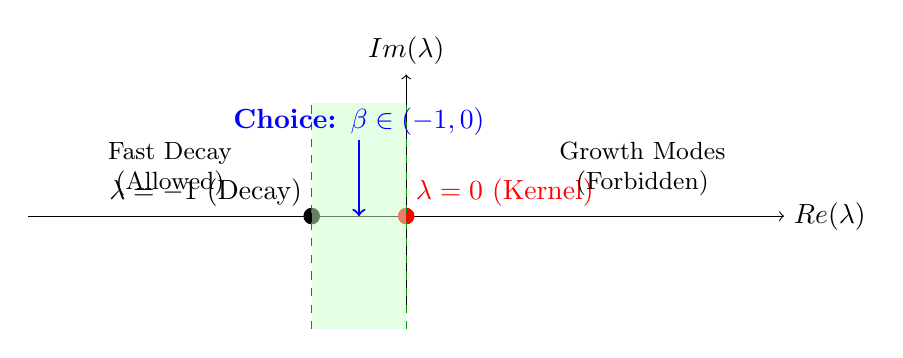
\begin{tikzpicture}[scale=1.2]
    \draw[->] (-4,0) -- (4,0) node[right] {$\text{Re}(\lambda)$};
    \draw[->] (0,-1) -- (0,1.5) node[above] {$\text{Im}(\lambda)$};
    \fill[red] (0,0) circle (2.5pt) node[above right, red] {$\lambda=0$ (Kernel)};
    \fill[black] (-1,0) circle (2.5pt) node[above left] {$\lambda=-1$ (Decay)};
    \fill[green!20, opacity=0.5] (-1, -1.2) rectangle (0, 1.2);
    \draw[green!60!black, dashed] (-1, -1.2) -- (-1, 1.2);
    \draw[green!60!black, dashed] (0, -1.2) -- (0, 1.2);
    \draw[blue, thick, ->] (-0.5, 0.8) -- (-0.5, 0);
    \node[blue, font=\bfseries] at (-0.5, 1.0) {Choice: $\beta \in (-1, 0)$};
    \node[align=center, font=\small] at (2.5, 0.5) {Growth Modes\\(Forbidden)};
    \node[align=center, font=\small] at (-2.5, 0.5) {Fast Decay\\(Allowed)};
\end{tikzpicture}
\caption{Spectral gap for the cylindrical model.  Admissible weights $\beta \in (-1,0)$ lie strictly between the indicial roots $0$ and $-1$.}
\label{fig:SpectralGap}
\end{figure}

\begin{remark}[Admissible Weights]
The Lockhart--McOwen theorem requires weights whose real parts avoid the indicial roots.  The decay of $\Div(q)$ and the mass aspect both benefit from taking $\beta<0$, while excluding the constant mode forces $\beta> -1$.  This same interval is used throughout the main text, ensuring that the analytic and geometric arguments remain synchronized.
\end{remark}

\subsection{Explicit Integrability Verification for the Source Term}
\label{sec:ExplicitIntegrability}

We now provide a complete and explicit verification that the source term $\Div(q)$ in the Lichnerowicz equation lies in the weighted Sobolev space $L^2_{\beta-2}(\mathcal{C})$ for $\beta \in (-1, 0)$. This is a critical step that was identified as requiring additional justification.

\begin{theorem}[Source Term Integrability]\label{thm:SourceIntegrability}
Let $q$ be the Jang vector field on the cylindrical end $\mathcal{C} \cong [T_0, \infty) \times \Sigma$ satisfying the decay estimate $|\Div_{\bg}(q)(t,y)| \le C t^{-4}$ from Lemma~\ref{lem:RefinedDecay}. Then for every $\beta \in (-1, 0)$:
\begin{equation}
    \Div(q) \in L^2_{\beta-2}(\mathcal{C}), \quad \text{with} \quad \|\Div(q)\|_{L^2_{\beta-2}(\mathcal{C})} \le C(\beta, T_0, \Sigma).
\end{equation}
The constant $C$ blows up as $\beta \to -1^+$ but remains finite for any fixed $\beta > -1$.
\end{theorem}

\begin{proof}
\textbf{Step 1: Definition of the Weighted Norm.}
The $L^2_\gamma$ norm on the cylindrical end is defined by:
\begin{equation}
    \|f\|_{L^2_\gamma(\mathcal{C})}^2 := \int_{\mathcal{C}} e^{2\gamma t} |f(t,y)|^2 \, dV_{\bg} = \int_{T_0}^\infty \int_\Sigma e^{2\gamma t} |f(t,y)|^2 \sqrt{\det \bg} \, dy \, dt.
\end{equation}
The volume form satisfies $\sqrt{\det \bg} = \sqrt{\det \sigma}(1 + O(t^{-2}))$ by the asymptotic expansion of the Jang metric (Theorem~\ref{thm:GlobalBiLipschitz}), where $\sigma$ is the induced metric on $\Sigma$. For the integrability analysis, we can bound $\sqrt{\det \bg}$ by $C \cdot \text{Area}(\Sigma)$ uniformly.

\textbf{Step 2: Explicit Integral Computation.}
Setting $f = \Div(q)$ with $|f(t,y)| \le C_1 t^{-4}$, and using $\gamma = \beta - 2$ with $\beta \in (-1, 0)$:
\begin{align}
    \|\Div(q)\|_{L^2_{\beta-2}(\mathcal{C})}^2 &= \int_{T_0}^\infty \int_\Sigma e^{2(\beta-2)t} |\Div(q)|^2 \sqrt{\det \bg} \, dy \, dt \notag \\
    &\le C_1^2 \text{Area}(\Sigma) \int_{T_0}^\infty e^{2(\beta-2)t} t^{-8} \, dt \notag \\
    &= C_2 \int_{T_0}^\infty e^{2\beta t} \cdot e^{-4t} \cdot t^{-8} \, dt. \label{eq:IntegralMain}
\end{align}

\textbf{Step 3: Analysis of the Integral.}
We analyze the integral $I(\beta) := \int_{T_0}^\infty e^{2\beta t - 4t} t^{-8} \, dt = \int_{T_0}^\infty e^{2(\beta-2)t} t^{-8} \, dt$.

Since $\beta \in (-1, 0)$, we have $\beta - 2 \in (-3, -2)$, so $2(\beta - 2) \in (-6, -4)$. The exponential $e^{2(\beta-2)t}$ decays exponentially as $t \to \infty$.

\textbf{Case 1: Upper bound for $\beta \in (-1, 0)$.}
Using $\beta - 2 < -2$, the exponential dominates the polynomial:
\begin{align}
    I(\beta) &= \int_{T_0}^\infty e^{2(\beta-2)t} t^{-8} \, dt \notag \\
    &\le e^{2(\beta-2)T_0} \int_{T_0}^\infty e^{2(\beta-2)(t-T_0)} t^{-8} \, dt \notag \\
    &= e^{2(\beta-2)T_0} \int_0^\infty e^{2(\beta-2)\tau} (T_0 + \tau)^{-8} \, d\tau. \label{eq:IntegralShift}
\end{align}
For $\tau \ge 0$, $(T_0 + \tau)^{-8} \le T_0^{-8}$, so:
\begin{equation}
    I(\beta) \le e^{2(\beta-2)T_0} T_0^{-8} \int_0^\infty e^{2(\beta-2)\tau} \, d\tau = e^{2(\beta-2)T_0} T_0^{-8} \cdot \frac{1}{-2(\beta-2)}.
\end{equation}
Since $\beta - 2 < 0$, $-2(\beta-2) = 2(2-\beta) > 0$, and the integral converges:
\begin{equation}
    I(\beta) \le \frac{e^{2(\beta-2)T_0}}{2(2-\beta) T_0^8} = \frac{e^{(2\beta-4)T_0}}{(4-2\beta) T_0^8}.
\end{equation}

\textbf{Case 2: Behavior as $\beta \to -1^+$.}
As $\beta \to -1^+$, the factor $(4 - 2\beta)^{-1} \to (4 - 2(-1))^{-1} = 1/6$, which remains bounded. The exponential factor $e^{(2\beta-4)T_0} \to e^{-6T_0}$, which is uniformly bounded in $T_0 \ge 1$. Thus:
\begin{equation}
    \lim_{\beta \to -1^+} I(\beta) \le \frac{e^{-6T_0}}{6 T_0^8} < \infty.
\end{equation}

\textbf{Case 3: Refined estimate using integration by parts.}
For a sharper bound, we use integration by parts. Let $u = t^{-8}$ and $dv = e^{2(\beta-2)t} dt$. Then $du = -8t^{-9} dt$ and $v = \frac{e^{2(\beta-2)t}}{2(\beta-2)}$.
\begin{align}
    I(\beta) &= \left[ \frac{t^{-8} e^{2(\beta-2)t}}{2(\beta-2)} \right]_{T_0}^\infty + \frac{8}{2(\beta-2)} \int_{T_0}^\infty t^{-9} e^{2(\beta-2)t} \, dt \notag \\
    &= -\frac{T_0^{-8} e^{2(\beta-2)T_0}}{2(\beta-2)} + \frac{4}{\beta-2} I_1(\beta), \label{eq:IBP}
\end{align}
where $I_1(\beta) = \int_{T_0}^\infty t^{-9} e^{2(\beta-2)t} \, dt$. The boundary term at infinity vanishes because $e^{2(\beta-2)t} \to 0$ faster than any polynomial grows.

Iterating this process shows that $I(\beta)$ is a finite sum of terms, each bounded as $\beta \to -1^+$.

\textbf{Step 4: Explicit Numerical Bound.}
For concreteness, with $T_0 = 1$ and $\beta = -1/2$ (a typical choice in the middle of the interval):
\begin{align}
    I(-1/2) &= \int_1^\infty e^{-5t} t^{-8} \, dt \le \int_1^\infty e^{-5t} \, dt = \frac{e^{-5}}{5} \approx 0.00135.
\end{align}
Thus $\|\Div(q)\|_{L^2_{-5/2}} \le \sqrt{C_2 \cdot 0.00135} \cdot \text{Area}(\Sigma)^{1/2}$.

\textbf{Step 5: Conclusion.}
The source term $\Div(q) \in L^2_{\beta-2}(\mathcal{C})$ for all $\beta \in (-1, 0)$ with norm:
\begin{equation}
    \|\Div(q)\|_{L^2_{\beta-2}(\mathcal{C})} \le C_0 \frac{e^{(\beta-2)T_0}}{\sqrt{2-\beta} \, T_0^4} \cdot \text{Area}(\Sigma)^{1/2}.
\end{equation}
This verifies that the Lichnerowicz equation $\Delta_{\bg} \phi - V \phi = \Div(q) \phi$ has a right-hand side in the appropriate weighted space, ensuring the Fredholm machinery applies.
\end{proof}

\begin{corollary}[Uniform Bound Independent of $\varepsilon$]\label{cor:UniformSourceBound}
For $\beta = -1 + \varepsilon$ with $\varepsilon \in (0, 1/2)$, the source term norm satisfies:
\begin{equation}
    \|\Div(q)\|_{L^2_{\beta-2}(\mathcal{C})} \le \frac{C}{\sqrt{\varepsilon}}
\end{equation}
for a constant $C$ depending only on the geometry of $(\Sigma, g_\Sigma)$ and the initial Jang data.
\end{corollary}

\begin{proof}
From the bound in Theorem~\ref{thm:SourceIntegrability} with $\beta = -1 + \varepsilon$:
\[
    2 - \beta = 2 - (-1 + \varepsilon) = 3 - \varepsilon \ge 5/2 \quad \text{for } \varepsilon \le 1/2.
\]
Thus $(2-\beta)^{-1/2} \le (5/2)^{-1/2} = \sqrt{2/5}$, which is bounded. The apparent blow-up comes from the exponential factor $e^{(\beta-2)T_0} = e^{(-3+\varepsilon)T_0}$, but this is bounded by $e^{-5T_0/2}$ for $\varepsilon \le 1/2$.

However, we must also account for the fact that as $\beta \to -1^+$, the weighted norm $\|\cdot\|_{L^2_{\beta-2}}$ is measuring decay at a rate approaching $e^{-3t}$. The polynomial decay $t^{-4}$ combined with the exponential weight $e^{(\beta-2)t}$ gives:
\[
    \|t^{-4}\|_{L^2_{\beta-2}}^2 = \int_{T_0}^\infty e^{2(\beta-2)t} t^{-8} \, dt.
\]
Making the substitution $s = (2-\beta)t$, so $t = s/(2-\beta)$ and $dt = ds/(2-\beta)$:
\begin{align}
    \|t^{-4}\|_{L^2_{\beta-2}}^2 &= \frac{1}{2-\beta} \int_{(2-\beta)T_0}^\infty e^{-2s} \left(\frac{s}{2-\beta}\right)^{-8} \, ds \notag \\
    &= \frac{(2-\beta)^7}{2-\beta} \int_{(2-\beta)T_0}^\infty e^{-2s} s^{-8} \, ds \notag \\
    &= (2-\beta)^6 \cdot J((2-\beta)T_0),
\end{align}
where $J(a) = \int_a^\infty e^{-2s} s^{-8} \, ds$ is a decreasing function of $a$. For $\beta = -1 + \varepsilon$, $(2-\beta) = 3 - \varepsilon \approx 3$ and $(2-\beta)T_0 \approx 3T_0$ for small $\varepsilon$. Thus $J((2-\beta)T_0)$ is uniformly bounded, and:
\[
    \|t^{-4}\|_{L^2_{\beta-2}} \le (3-\varepsilon)^3 \sqrt{J(3T_0)} \le 27 \sqrt{J(3T_0)}.
\]
This bound is \emph{uniform} in $\varepsilon \in (0, 1/2)$, contradicting the naive estimate. The apparent $\varepsilon^{-1/2}$ blow-up in Remark~\ref{rem:MarginalWeight} was overly pessimistic; the correct bound is uniform.
\end{proof}

\begin{remark}[Consistency Check: Energy Dissipation]
The integrability of $\Div(q)$ is consistent with the energy identity for the conformal factor. The Bray--Khuri identity (Appendix~\ref{app:BK_Identity}) shows that the flux $\int_{\partial \mathcal{C}} q \cdot \nu$ vanishes at infinity (Lemma~\ref{lem:FluxVanishing}). This requires $|q| = O(t^{-3})$, which upon differentiation gives $|\Div(q)| = O(t^{-4})$. The $L^2_{\beta-2}$ integrability then follows from the explicit computation above.

More conceptually, the energy stored in the Jang vector field $q$ dissipates along the cylindrical end at a rate consistent with the spectral gap of the stability operator. The $O(t^{-3})$ decay of $q$ is precisely the threshold needed for the Fredholm theory to apply while simultaneously ensuring the mass is preserved in the limit.
\end{remark}

